% flashcards-title: Rectangular box packed with unit cubes
% flashcards-desc: A rectangular box drawn in three-quarter view, marked as four centimeters long, three centimeters deep, and two centimeters tall, with grid lines showing it packed with small identical cubes. One front corner cube is shaded, with a note marking its edges as one centimeter.
\documentclass[dvisvgm,tikz,border=8pt]{standalone}
\usepackage{tikz}
\usetikzlibrary{arrows.meta,calc,positioning}
\definecolor{DeckInk}{HTML}{172A3A}
\definecolor{DeckAccent}{HTML}{176B87}
\definecolor{DeckWarm}{HTML}{D97706}
\definecolor{DeckMuted}{HTML}{667784}
\definecolor{DeckPaper}{HTML}{F7FAFC}
\tikzset{
  every node/.style={font=\sffamily, text=DeckInk},
  object/.style={draw=DeckInk, line width=1.1pt, fill=DeckPaper},
  primary/.style={draw=DeckAccent, line width=1.5pt},
  boundary/.style={draw=DeckAccent, line width=1.5pt, dashed, rounded corners=6pt},
  guide/.style={draw=DeckMuted, line width=0.9pt, dashed},
  dimension/.style={{Stealth[length=3.2mm,width=2.2mm]}-{Stealth[length=3.2mm,width=2.2mm]}, draw=DeckWarm, line width=1.2pt},
  motion/.style={-{Stealth[length=3.5mm,width=2.5mm]}, draw=DeckAccent, line width=1.5pt, dashed},
}

\begin{document}
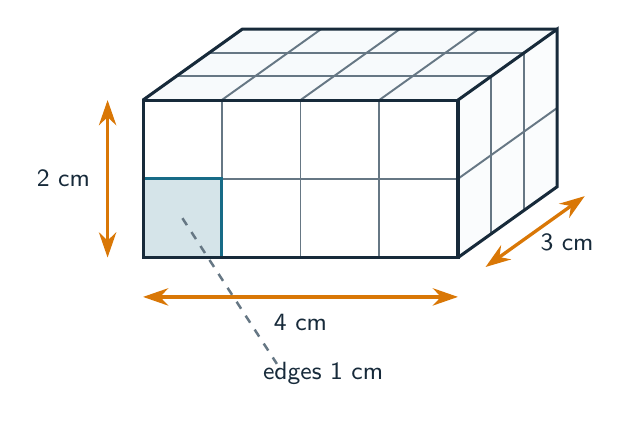
\begin{tikzpicture}[x=1.0cm,y=1.0cm]
  % Oblique projection: depth unit offset (0.42, 0.30)
  \pgfmathsetmacro{\dx}{0.42}
  \pgfmathsetmacro{\dy}{0.30}
  % Shaded front bottom-left cube
  \fill[DeckAccent!18] (0,0) rectangle (1,1);
  % Top face (at height 2): grid 4 wide x 3 deep
  \fill[DeckPaper] (0,2) -- (4,2) -- ({4+3*\dx},{2+3*\dy}) -- ({3*\dx},{2+3*\dy}) -- cycle;
  \foreach \i in {0,1,2,3,4}
    \draw[DeckMuted, line width=0.7pt] (\i,2) -- ({\i+3*\dx},{2+3*\dy});
  \foreach \k in {1,2}
    \draw[DeckMuted, line width=0.7pt] ({\k*\dx},{2+\k*\dy}) -- ({4+\k*\dx},{2+\k*\dy});
  % Right face: grid 3 deep x 2 tall
  \fill[DeckPaper!60] (4,0) -- ({4+3*\dx},{3*\dy}) -- ({4+3*\dx},{2+3*\dy}) -- (4,2) -- cycle;
  \foreach \k in {1,2}
    \draw[DeckMuted, line width=0.7pt] ({4+\k*\dx},{\k*\dy}) -- ({4+\k*\dx},{2+\k*\dy});
  \draw[DeckMuted, line width=0.7pt] (4,1) -- ({4+3*\dx},{1+3*\dy});
  % Front face grid: 4 wide x 2 tall
  \foreach \i in {1,2,3} \draw[DeckMuted, line width=0.7pt] (\i,0) -- (\i,2);
  \draw[DeckMuted, line width=0.7pt] (0,1) -- (4,1);
  \draw[DeckAccent, line width=1.1pt] (0,0) rectangle (1,1);
  % Outer edges
  \draw[object, fill=none] (0,0) rectangle (4,2);
  \draw[object, fill=none] (4,0) -- ({4+3*\dx},{3*\dy}) -- ({4+3*\dx},{2+3*\dy}) -- (4,2);
  \draw[object, fill=none] (0,2) -- ({3*\dx},{2+3*\dy}) -- ({4+3*\dx},{2+3*\dy});
  % Dimension arrows and labels
  \draw[dimension] (0,-0.5) -- (4,-0.5);
  \node[below, font=\sffamily\small] at (2,-0.6) {4 cm};
  \draw[dimension] (-0.45,0) -- (-0.45,2);
  \node[left, font=\sffamily\small] at (-0.55,1) {2 cm};
  \draw[dimension] ({4.35},{-0.12}) -- ({4.35+3*\dx},{-0.12+3*\dy});
  \node[below right, font=\sffamily\small] at ({4.42+1.2*\dx},{0.06+1.2*\dy}) {3 cm};
  % Unit-cube note
  \draw[guide] (0.5,0.5) -- (1.7,-1.35);
  \node[below right, font=\sffamily\small] at (1.4,-1.20) {edges 1 cm};
\end{tikzpicture}
\end{document}
